The simulation experiments served a vital role in the validation and enhancement of the algorithm. The primary objective was to verify the functionality of the algorithm's design and implementation of individual parts. Secondly, the experiments were designed to identify areas of improvement within our algorithm. Lastly, creating diverse scenarios allowed us to test and assess the algorithm's performance in different situations.\\

\section{Algorithm functionality experiments}
    The first runs of simulation experiments were focused on testing the execution capabilities of the algorithm. They aimed to verify the node's stability, testing if they would crash or stall the execution of the algorithm. These experiments served a major role in exposing errors in the implementation of our nodes and were instrumental in ensuring the stability of our solution.\\
    Moreover, we were able to detect several mistakes and places for improvement in the design of the algorithm's BT structure. The \texttt{Groot} application's log viewer was an invaluable tool for detecting these weak spots. The screen of the log viewer is shown in \ref{fig:log_viewer}.\\
    \begin{figure}[ht]
        \centering
        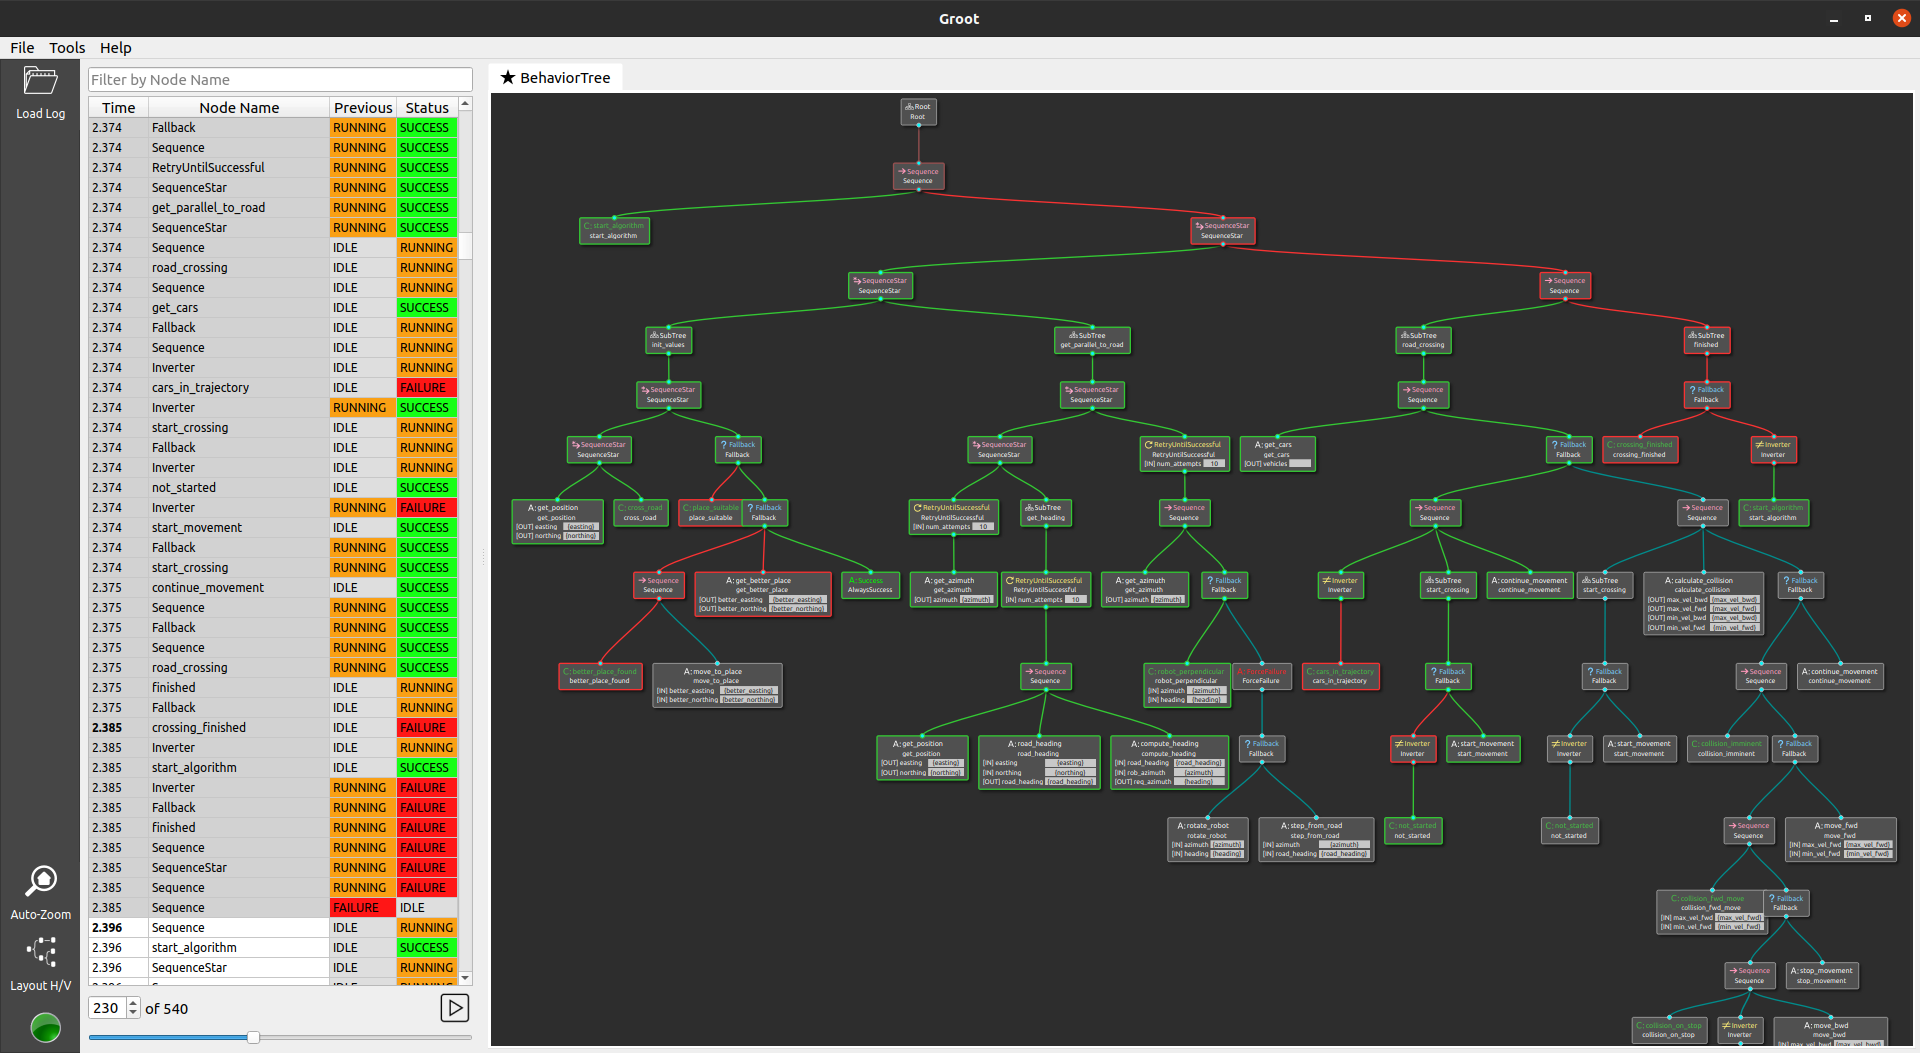
\includegraphics[width=\linewidth]{images/log_viewer.png}
        \caption{Log viewer in \texttt{Groot} application.}
        \label{fig:log_viewer}
    \end{figure}

\section{Algorithm behavior experiments}
    Once the stability of our algorithm was verified, we proceeded to test its behavior in different scenarios. We created several settings, each with a different configuration of the environment. With these scenarios, we tested the optimality and universality of our algorithm.\\
    We will present a few of the scenarios we created and discuss the results of the experiments and their importance within the validation process.\\
    We will present multiple figures with the settings of the vehicles relative to the robot. All used units correspond to the ones defined in section \ref{sec:Crossing-BT-impl}. The distances between objects are relative and not absolute. Also, if acceleration is not specified, it is assumed to be zero.\\
    \subsection{Used metrics}
        One of our tasks in the thesis assignement was to propose a metric for measuring the optimality of the robot's movement. The metric we created and used for evaluation is presented in this section.\\
        With each simulation experiment, we will present two graphs. One graph will show the minimal distance between the circumscribed rectangles of the robot and the vehicle. The second graph will show the velocities of the robot during its movement.\\
        The minimal distance between the circumscribed rectangles of the robot and the vehicle is a good metric for measuring the safety of the robot's movement. The smaller the distance, the higher the risk of collision.\\
        The velocities of the robot are a good metric for measuring the optimality of the robot's movement. The higher the velocity, the faster the robot will reach its goal.\\
        Other useful metrics for measuring the optimality of the robot's movement are the time it would take the robot to cross the road should it be empty and the time it took to cross the road in the given scenario. Another parameter is whether the robot was able to cross the road. And lastly, the minimal and average time to collision and the difference from start time to collision.\\
        The time to collision represents the estimated duration it would take for the robot to collide with the vehicle, assuming the robot maintains its current trajectory while the vehicle comes to a stop. The average time will be calculated from all relevant measurements. It would be pointless to calculate the time of collision if such collision is not possible.\\
        The deviation from the initial time to collision refers to the amount of time the robot would need to adjust the start time of its movement to ensure a collision occurs.
    \subsection{Simulation scenarios and results}
        \bfc{Scenario 1}\\
            The environment of the first scenario is shown in figure \ref{fig:scene1}. The goal of this simulation is to test the algorithm's capabilities of calculating the optimal velocities for the robot. As this was our first proper experiment, the condition node determining if the road was crossed were also tested.\\
            \begin{figure}[ht]
                \centering
                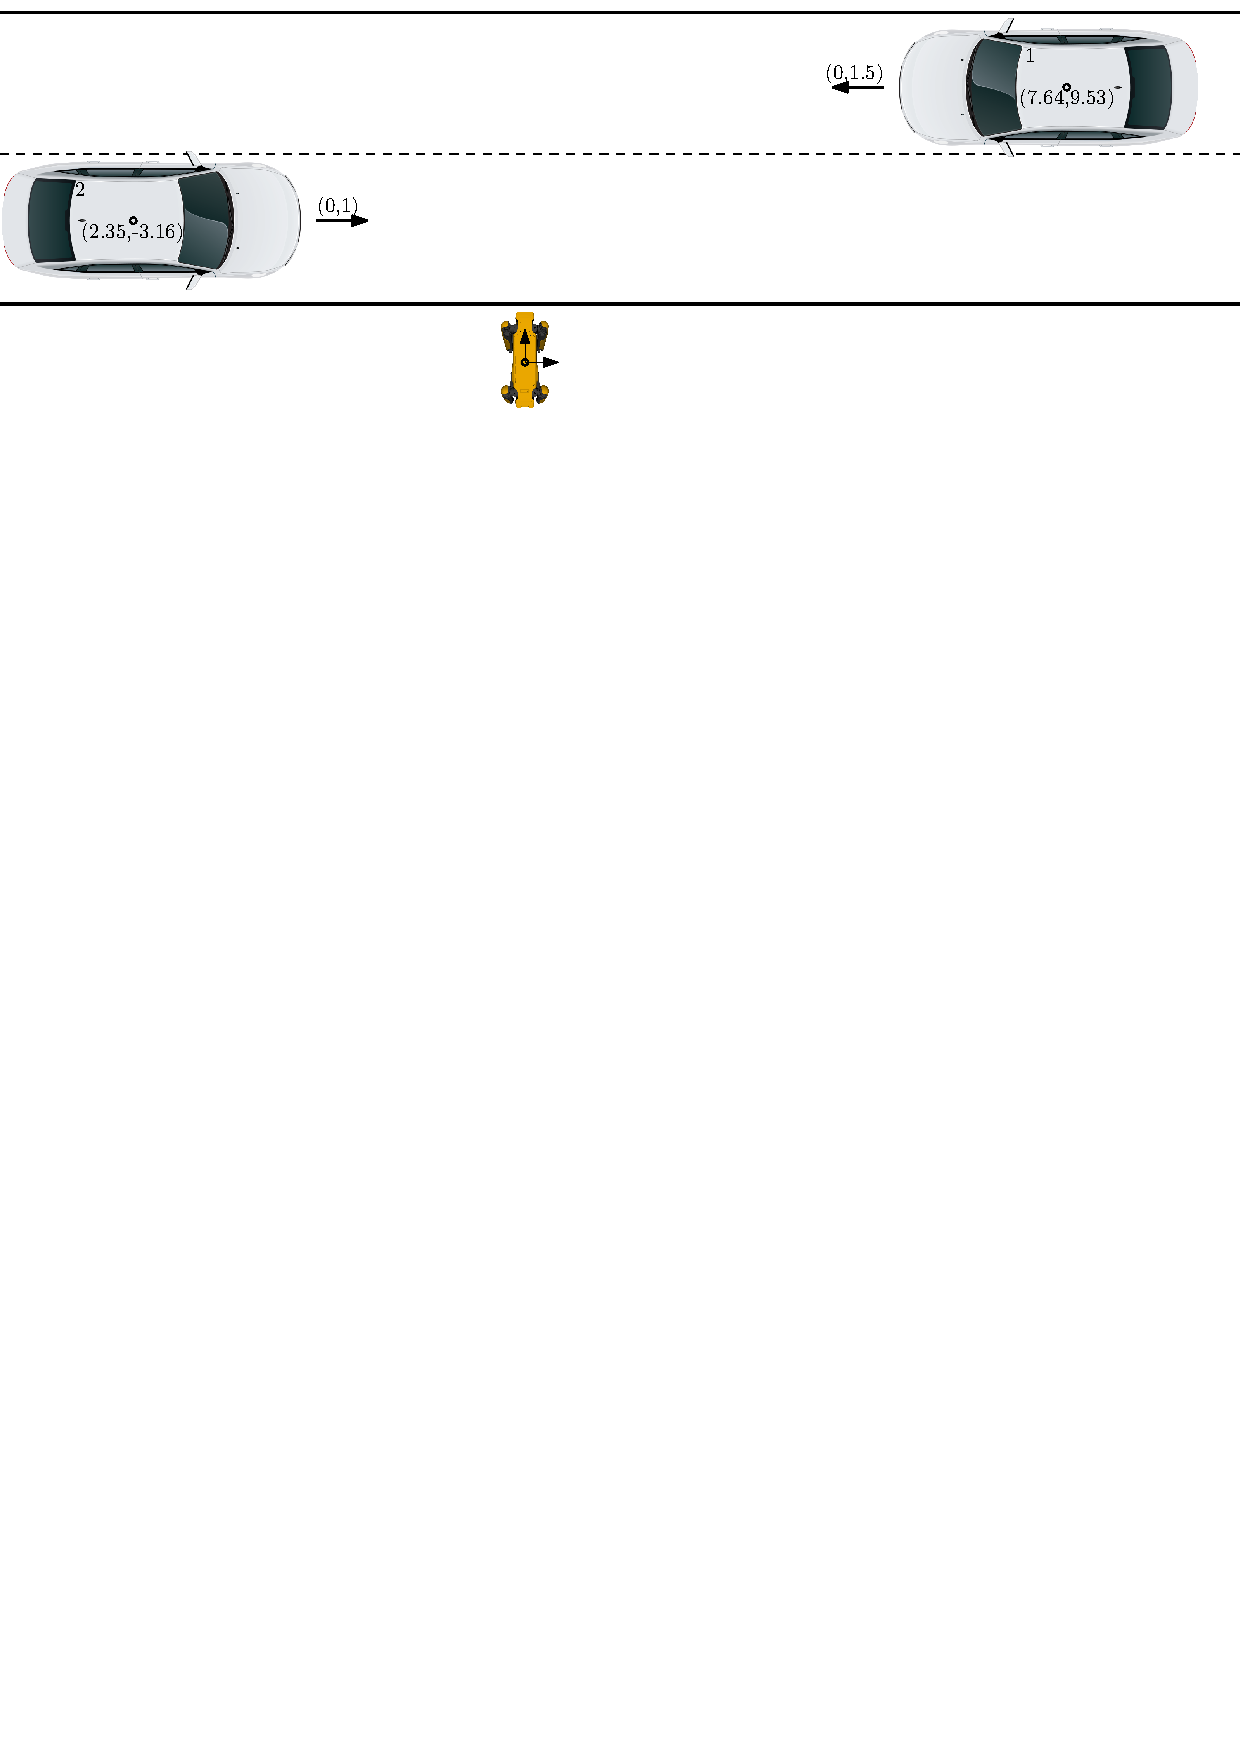
\includegraphics[width=\linewidth]{images/simulations/scene1.pdf}
                \caption{Environment for the first simulation scenario.}
                \label{fig:scene1}
            \end{figure}
            The graphs detailing the results of the experiment are shown in figure \ref{fig:scene1_graphs}.
            \begin{figure}[ht]
                \centering
                \begin{subfigure}{0.49\linewidth}
                    \centering
                    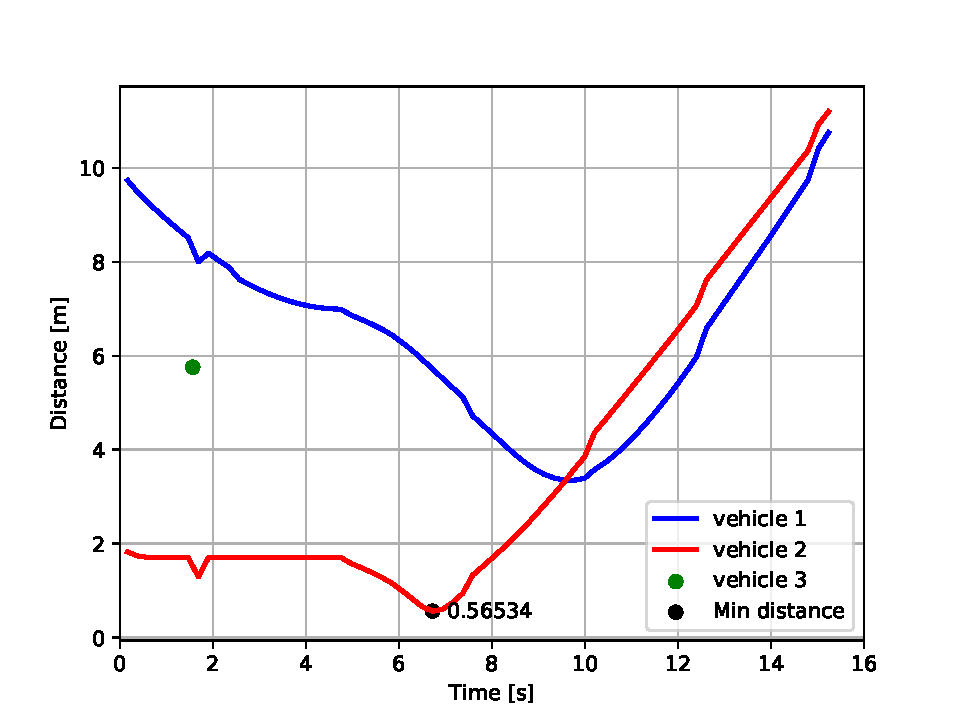
\includegraphics[trim={24 8 40 41}, clip, width=\linewidth]{images/simulations/scene1_dist.pdf}
                    \caption{Minimal distance between the robot and vehicles.}
                \end{subfigure}
                \begin{subfigure}{0.49\linewidth}
                    \centering
                    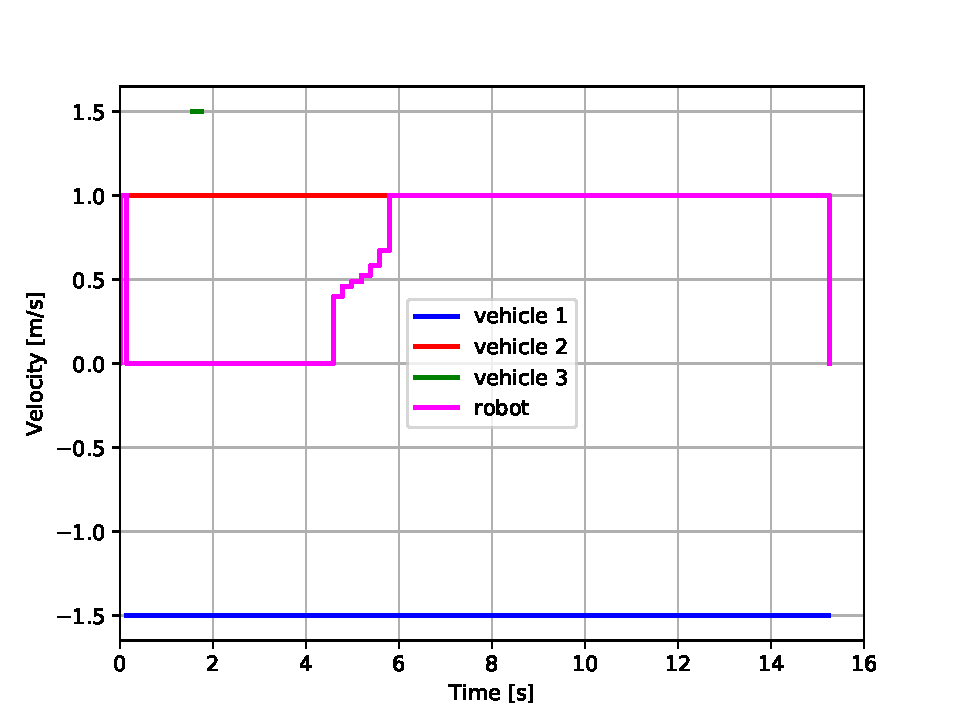
\includegraphics[trim={21 8 40 41}, clip, width=\linewidth]{images/simulations/scene1_vel.pdf}
                    \caption{Velocities of the robot during the crossing.}
                \end{subfigure}
                \caption{Results for the first scenarion of simulation experiments.}
                \label{fig:scene1_graphs}
            \end{figure}
        \bfc{Scenario 2}\\
            \begin{figure}[ht]
                \centering
                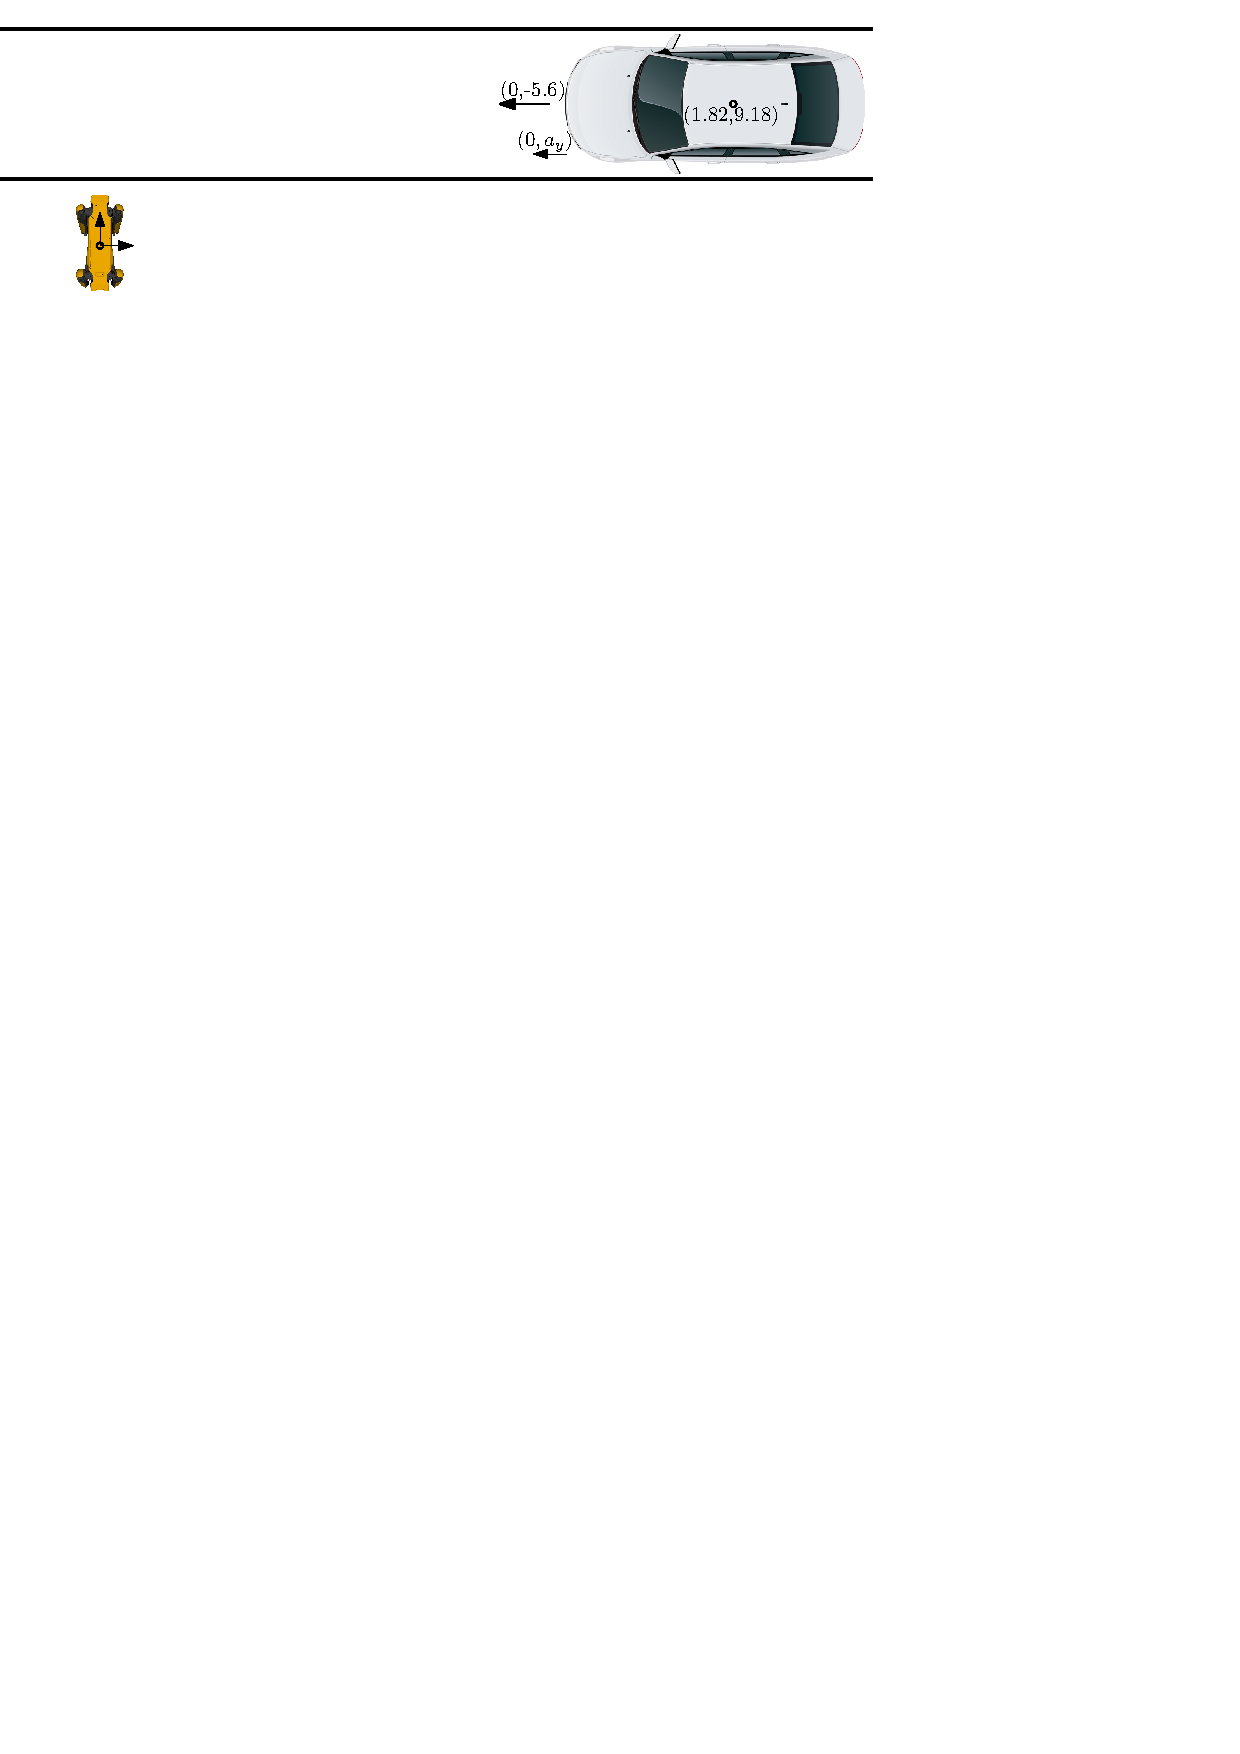
\includegraphics[width=\linewidth]{images/simulations/scene2.pdf}
                \caption{Environment for the second simulation scenario.}
                \label{fig:scene2}
            \end{figure}
            \begin{figure}[ht]
                \centering
                \begin{subfigure}{0.49\linewidth}
                    \centering
                    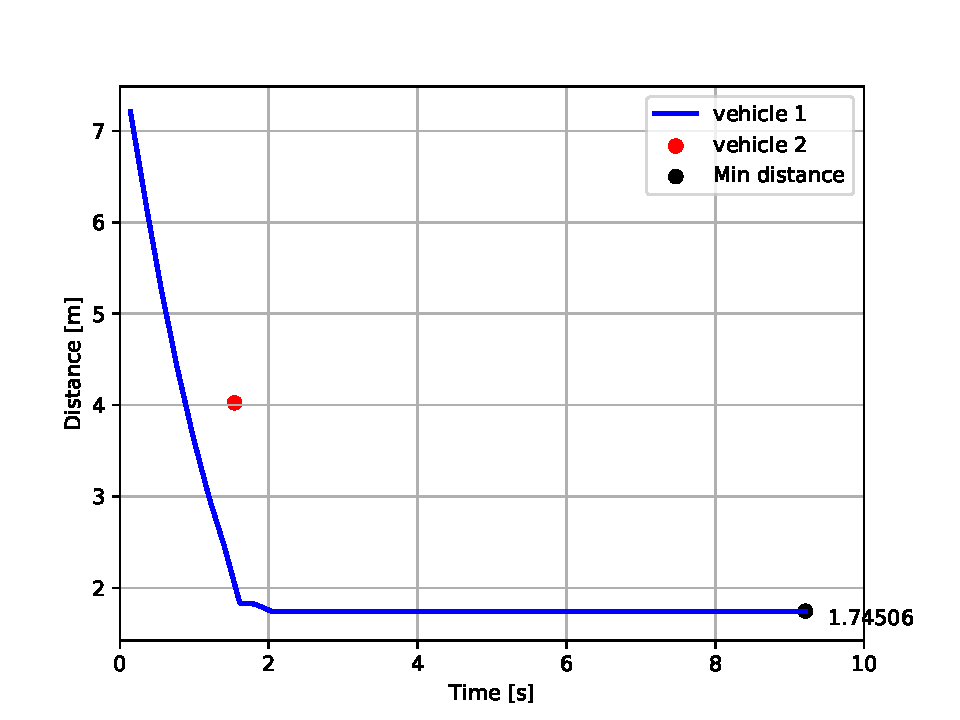
\includegraphics[trim={24 8 35 41}, clip, width=\linewidth]{images/simulations/scene2_1_dist.pdf}
                    \caption{Minimal distance between the robot and vehicles.}
                \end{subfigure}
                \begin{subfigure}{0.49\linewidth}
                    \centering
                    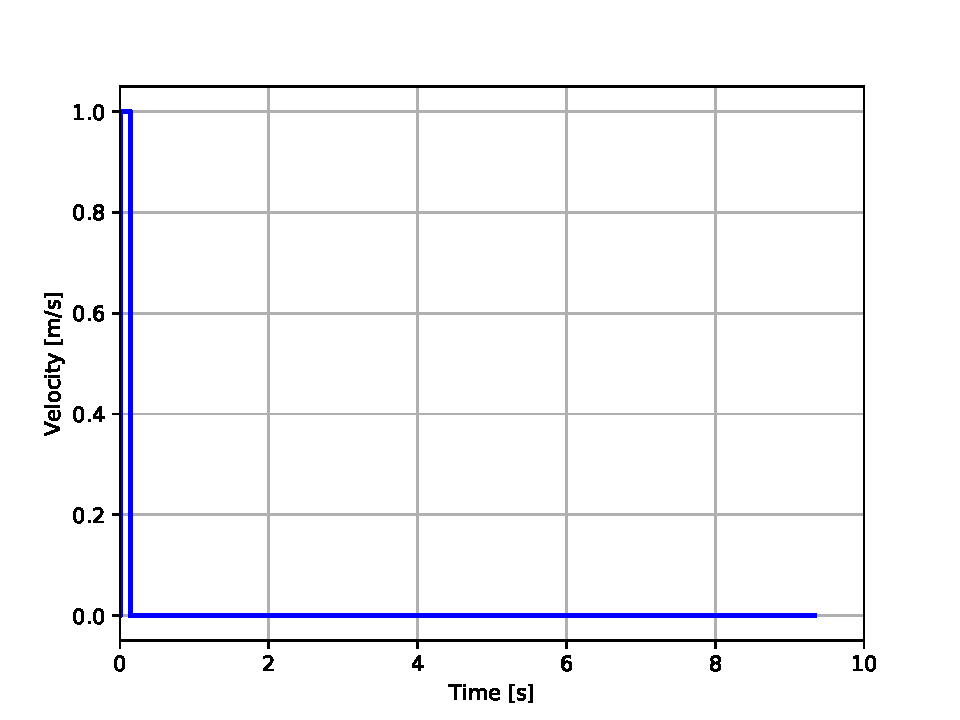
\includegraphics[trim={21 8 40 41}, clip, width=\linewidth]{images/simulations/scene2_1_vel.pdf}
                    \caption{Velocities of the robot during the crossing.}
                \end{subfigure}
                \caption{Results for the second scenarion of simulation experiments.}
                \label{fig:scene2_1_graphs}
            \end{figure}
            \begin{figure}[ht]
                \centering
                \begin{subfigure}{0.49\linewidth}
                    \centering
                    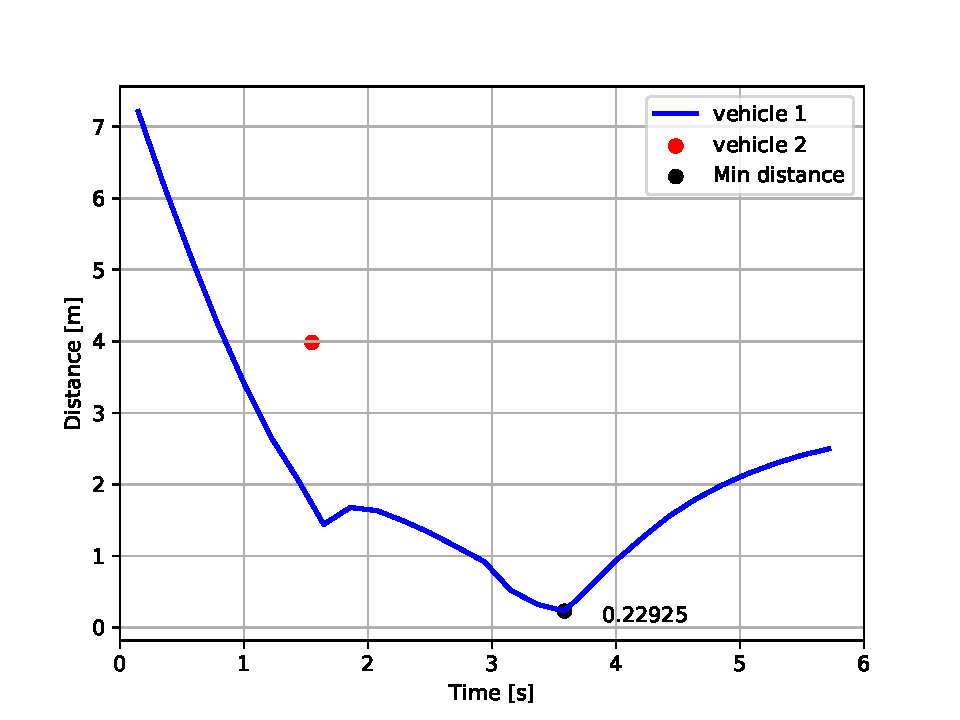
\includegraphics[trim={24 8 40 41}, clip, width=\linewidth]{images/simulations/scene2_2_dist.pdf}
                    \caption{Minimal distance between the robot and vehicles.}
                \end{subfigure}
                \begin{subfigure}{0.49\linewidth}
                    \centering
                    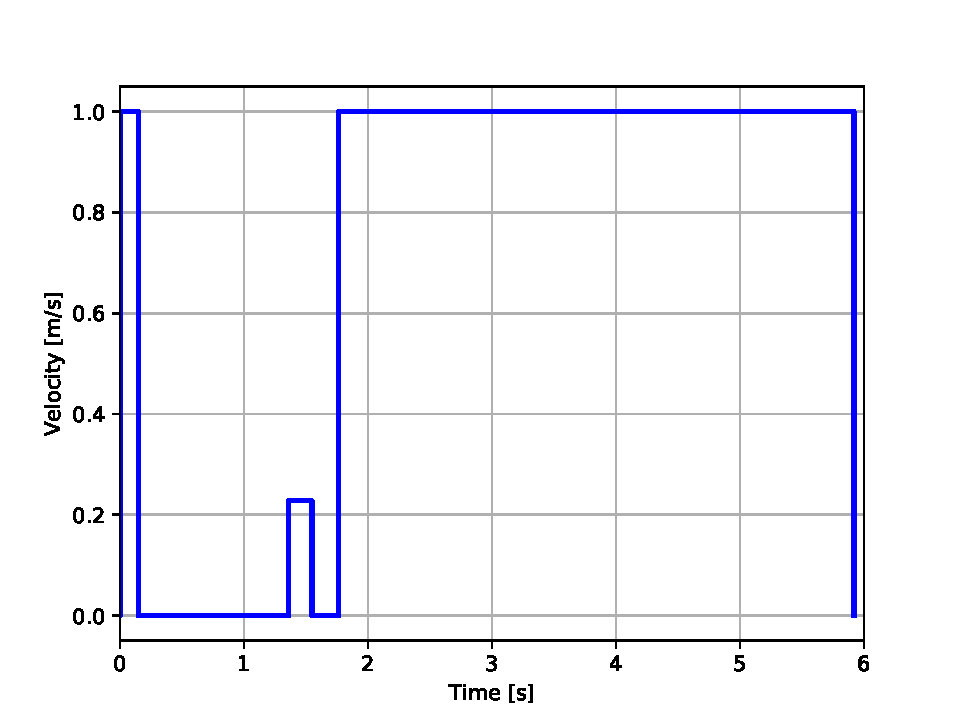
\includegraphics[trim={21 8 40 41}, clip, width=\linewidth]{images/simulations/scene2_2_vel.pdf}
                    \caption{Velocities of the robot during the crossing.}
                \end{subfigure}
                \caption{Results for the second scenarion of simulation experiments.}
                \label{fig:scene2_2_graphs}
            \end{figure}
            \begin{figure}[ht]
                \centering
                \begin{subfigure}{0.49\linewidth}
                    \centering
                    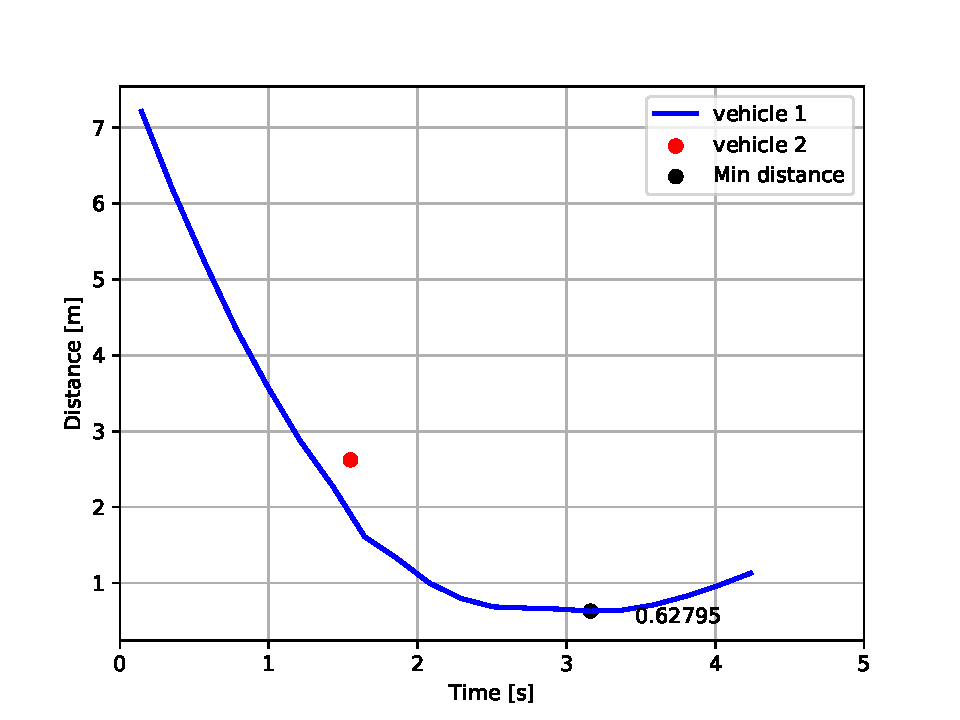
\includegraphics[trim={24 8 40 41}, clip, width=\linewidth]{images/simulations/scene2_3_dist.pdf}
                    \caption{Minimal distance between the robot and vehicles.}
                \end{subfigure}
                \begin{subfigure}{0.49\linewidth}
                    \centering
                    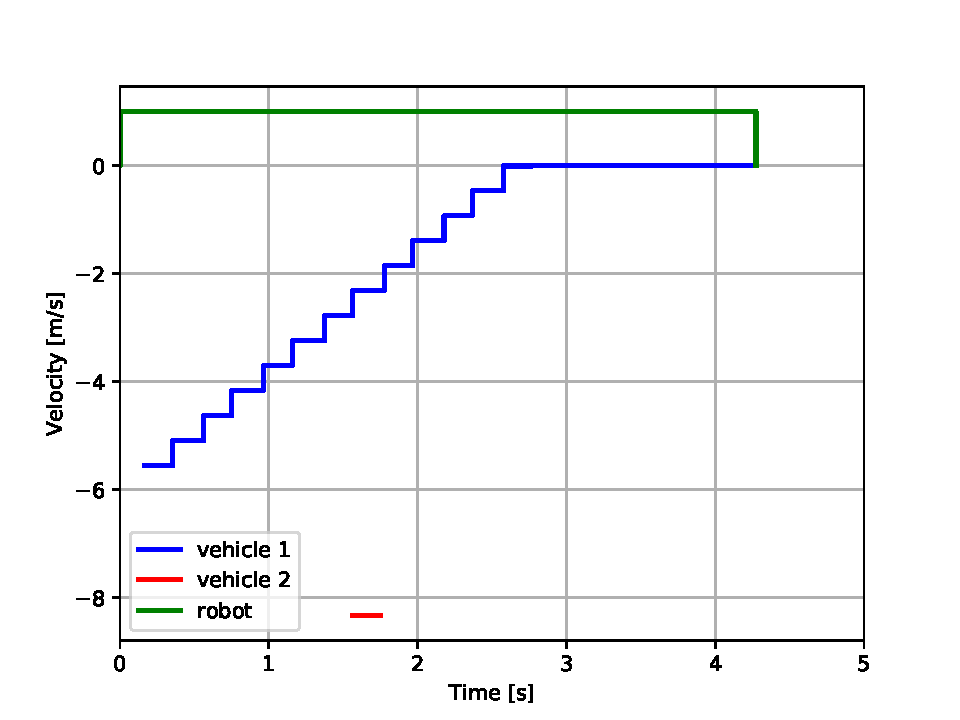
\includegraphics[trim={21 8 40 41}, clip, width=\linewidth]{images/simulations/scene2_3_vel.pdf}
                    \caption{Velocities of the robot during the crossing.}
                \end{subfigure}
                \caption{Results for the second scenarion of simulation experiments.}
                \label{fig:scene2_3_graphs}
            \end{figure}
        \bfc{Scenario 3}\\
            \begin{figure}[ht]
                \centering
                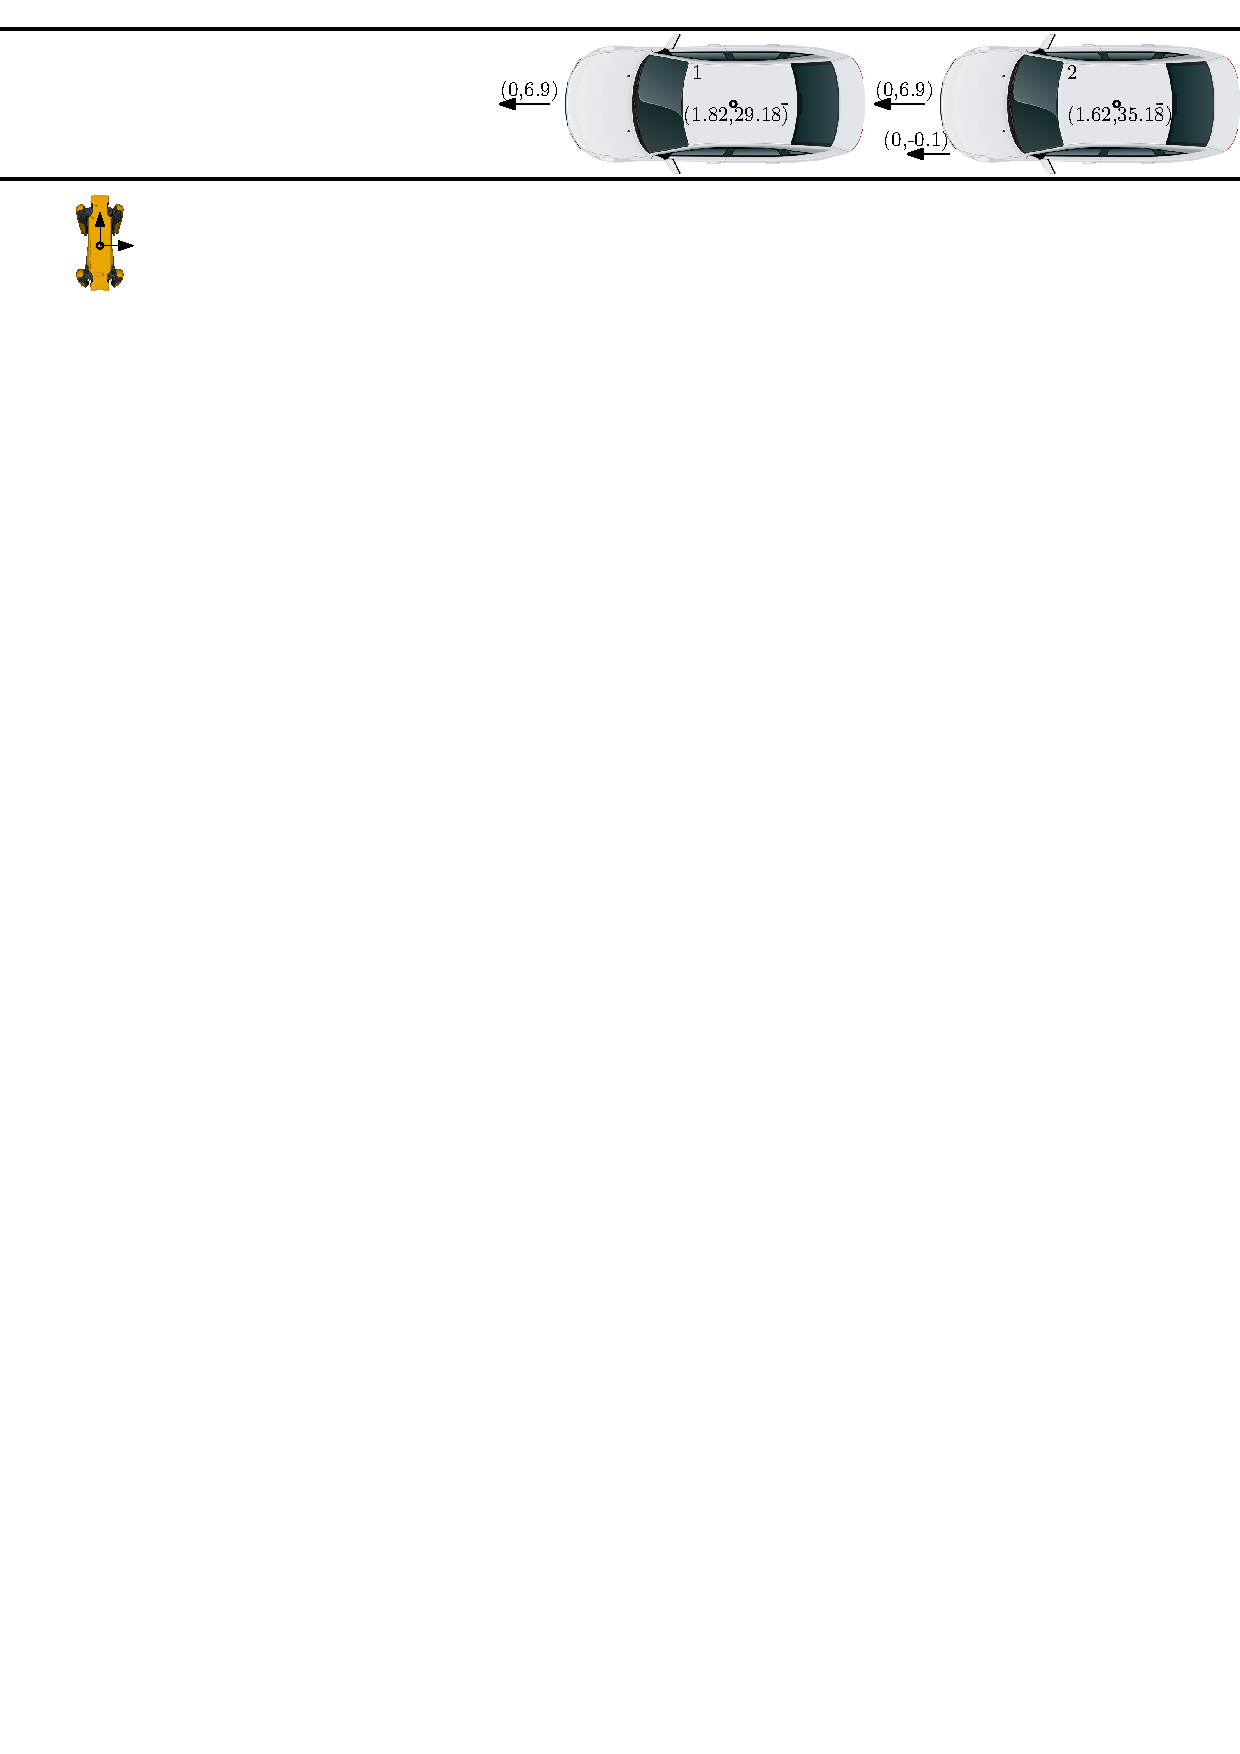
\includegraphics[width=\linewidth]{images/simulations/scene3.pdf}
                \caption{Environment for the third simulation scenario.}
                \label{fig:scene3}
            \end{figure}
            \begin{figure}[ht]
                \centering
                \begin{subfigure}{0.49\linewidth}
                    \centering
                    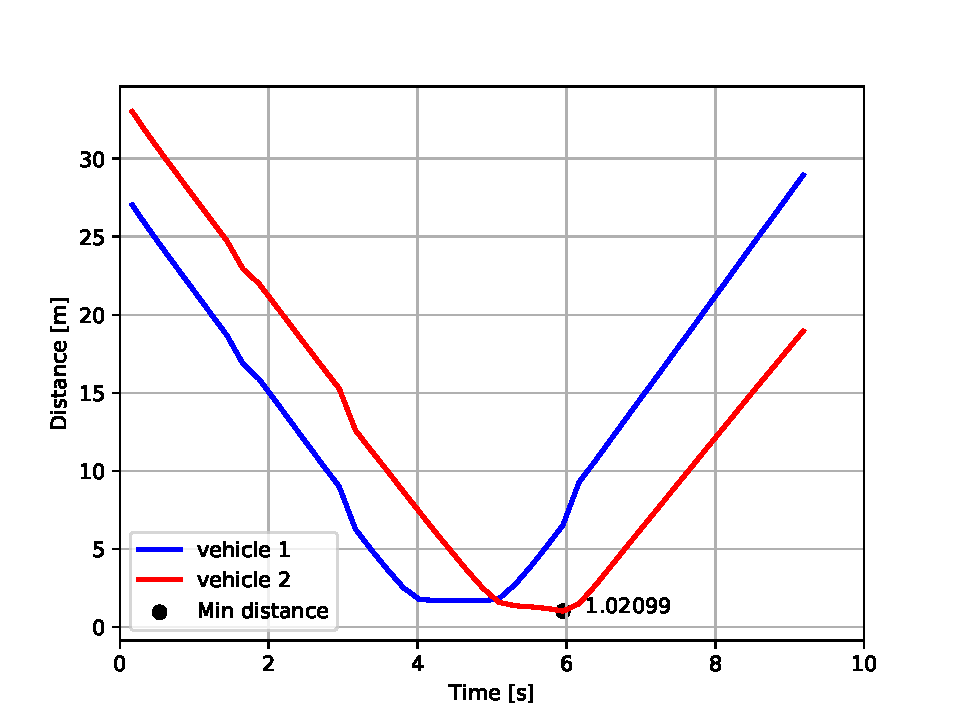
\includegraphics[trim={24 8 40 41}, clip, width=\linewidth]{images/simulations/scene3_dist.pdf}
                    \caption{Minimal distance between the robot and vehicles.}
                \end{subfigure}
                \begin{subfigure}{0.49\linewidth}
                    \centering
                    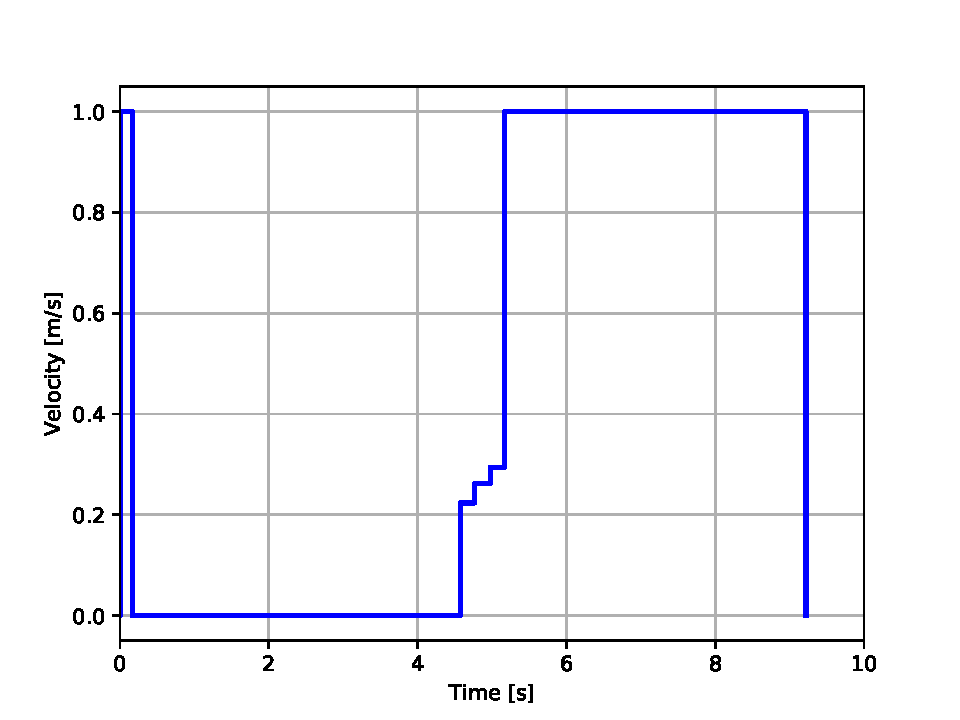
\includegraphics[trim={21 8 40 41}, clip, width=\linewidth]{images/simulations/scene3_vel.pdf}
                    \caption{Velocities of the robot during the crossing.}
                \end{subfigure}
                \caption{Results for the third scenarion of simulation experiments.}
                \label{fig:scene3_graphs}
            \end{figure}
        \bfc{Scenario 4}\\
            \begin{figure}[ht]
                \centering
                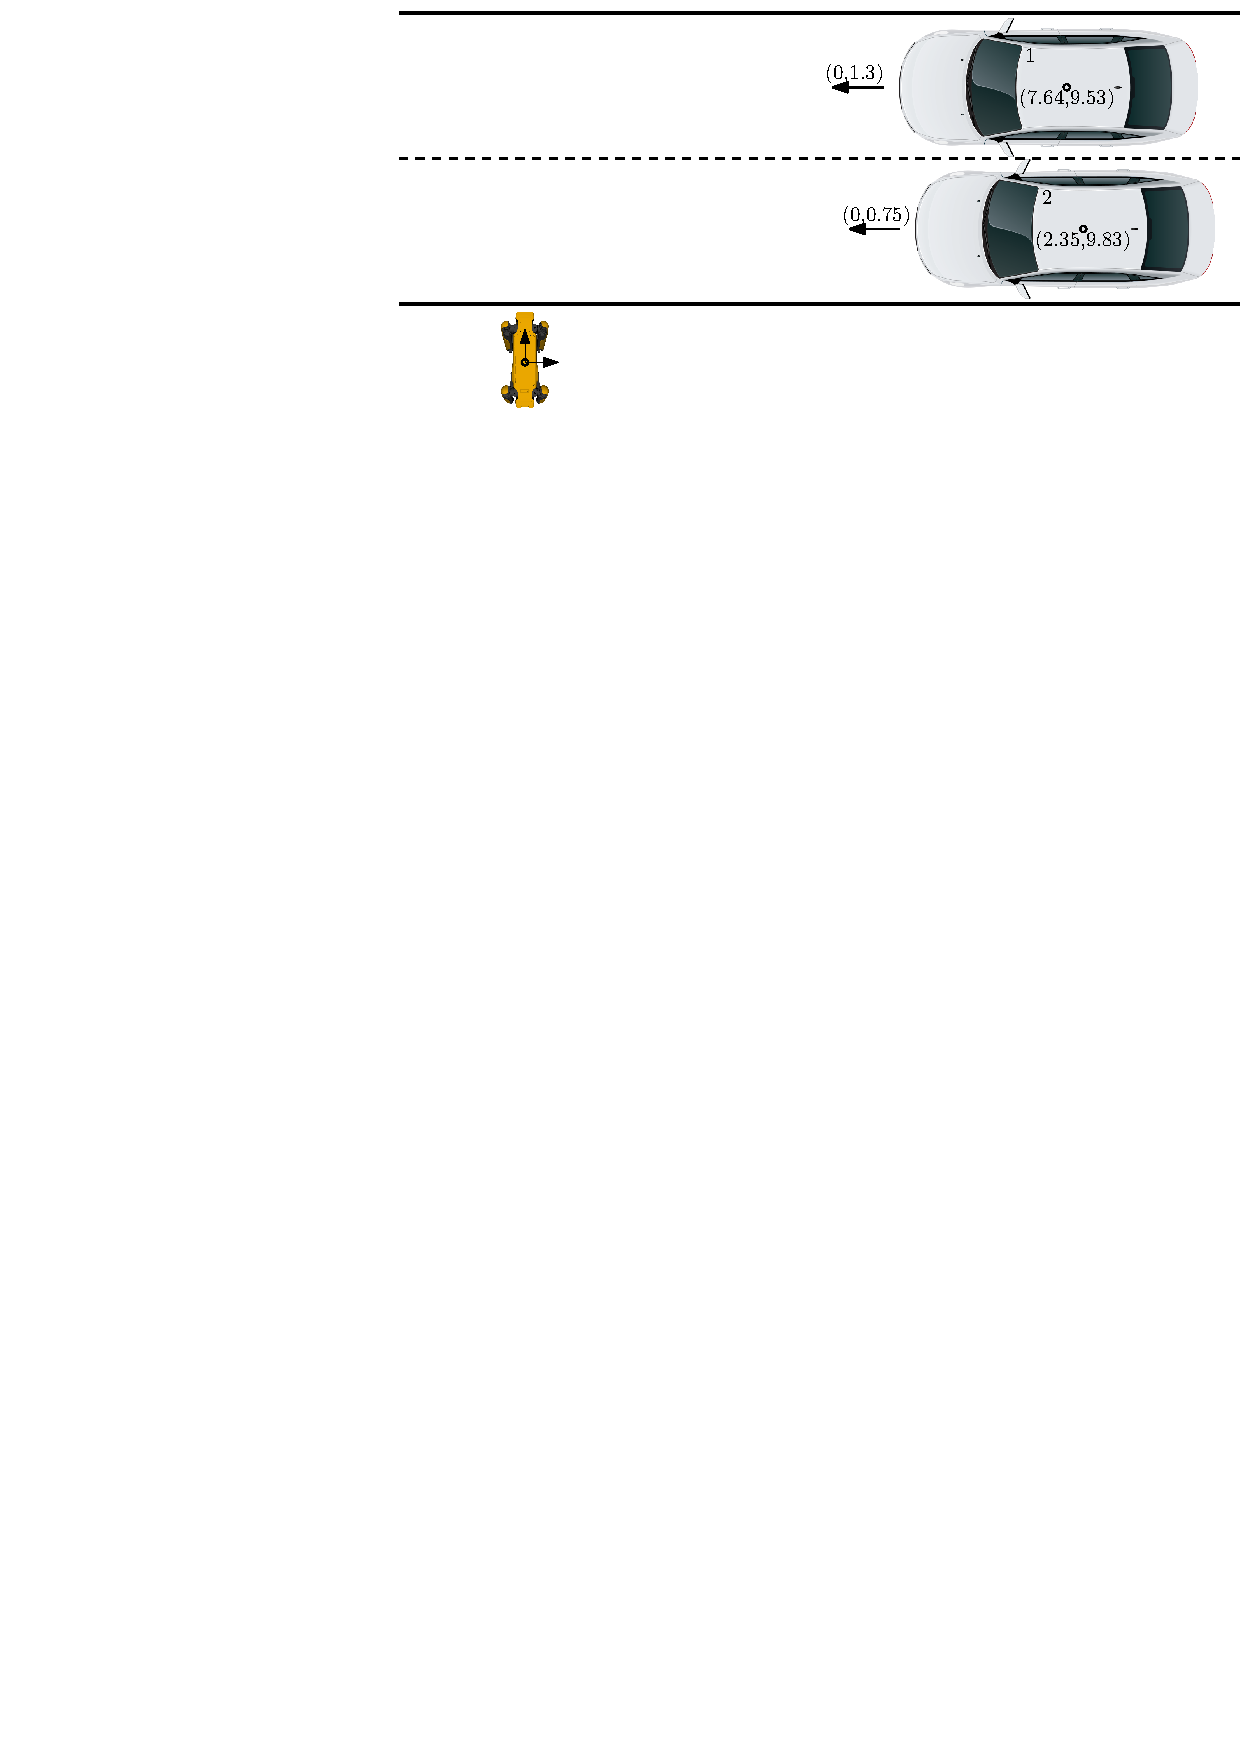
\includegraphics[width=\linewidth]{images/simulations/scene4.pdf}
                \caption{Environment for the fourth simulation scenario.}
                \label{fig:scene4}
            \end{figure}
            \begin{figure}[ht]
                \centering
                \begin{subfigure}{0.49\linewidth}
                    \centering
                    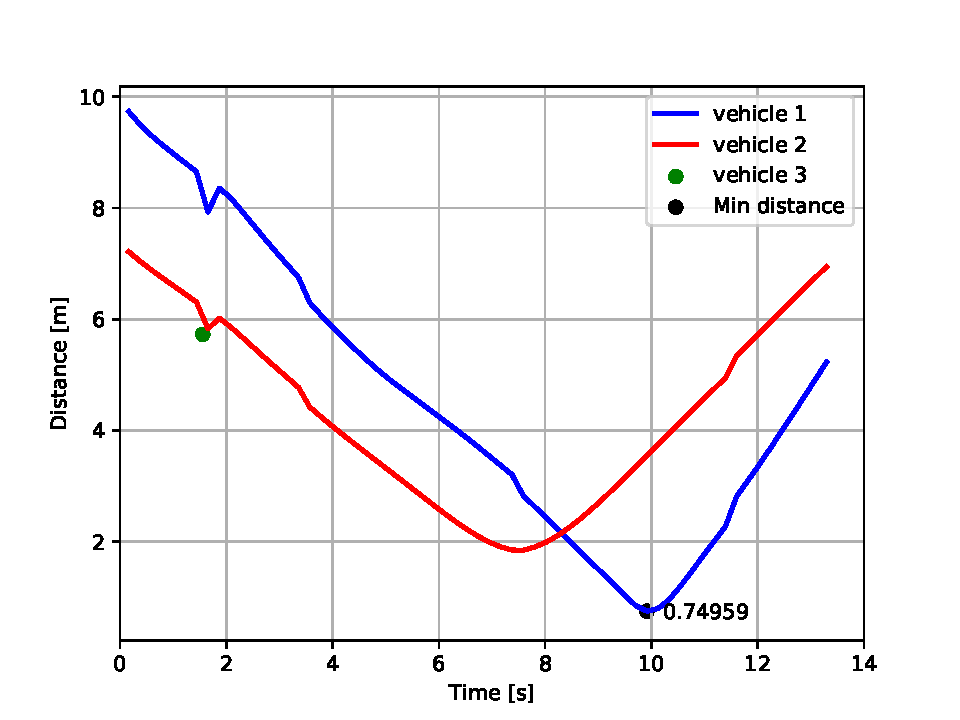
\includegraphics[trim={24 8 40 41}, clip, width=\linewidth]{images/simulations/scene4_1_dist.pdf}
                    \caption{Minimal distance between the robot and vehicles.}
                \end{subfigure}
                \begin{subfigure}{0.49\linewidth}
                    \centering
                    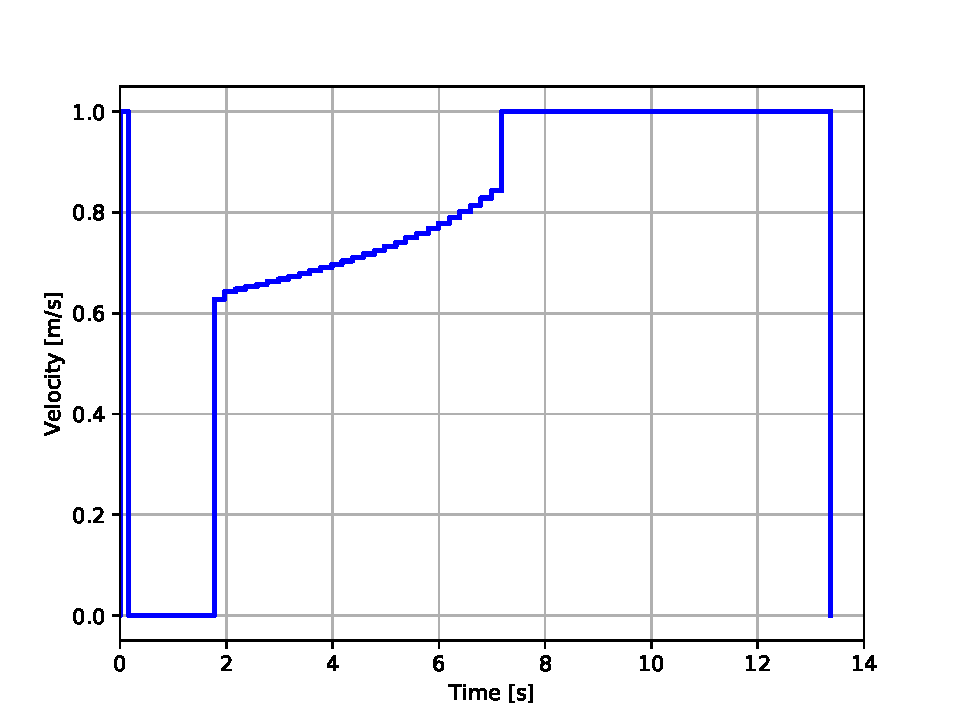
\includegraphics[trim={21 8 40 41}, clip, width=\linewidth]{images/simulations/scene4_1_vel.pdf}
                    \caption{Velocities of the robot during the crossing.}
                \end{subfigure}
                \caption{Results for the fourth scenarion of simulation experiments.}
                \label{fig:scene4_1_graphs}
            \end{figure}
            \begin{figure}[ht]
                \centering
                \begin{subfigure}{0.49\linewidth}
                    \centering
                    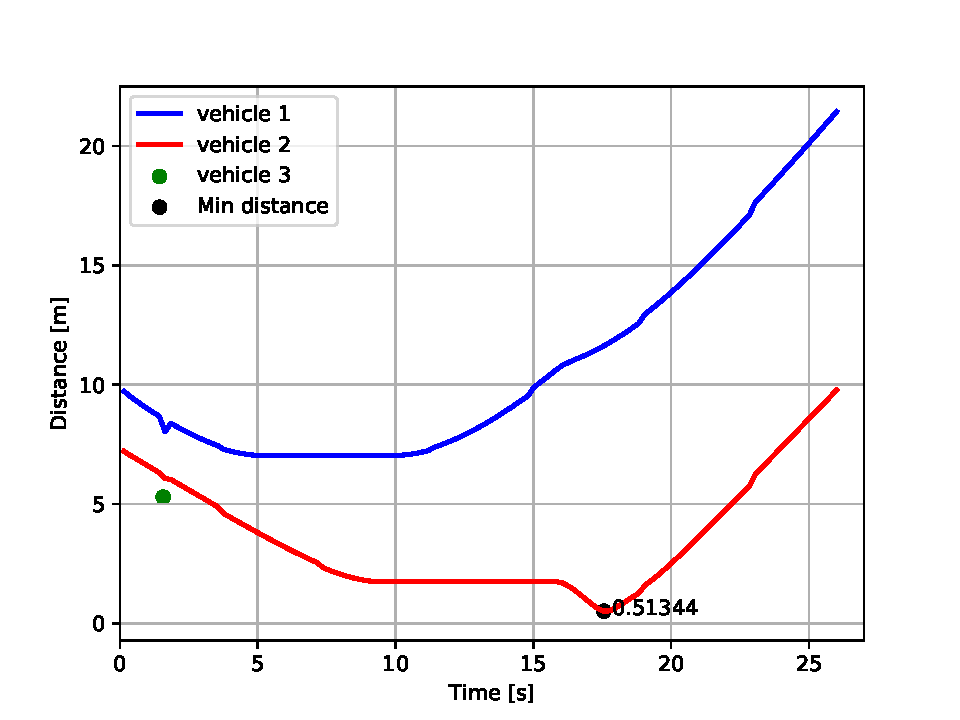
\includegraphics[trim={24 8 40 41}, clip, width=\linewidth]{images/simulations/scene4_2_dist.pdf}
                    \caption{Minimal distance between the robot and vehicles.}
                \end{subfigure}
                \begin{subfigure}{0.49\linewidth}
                    \centering
                    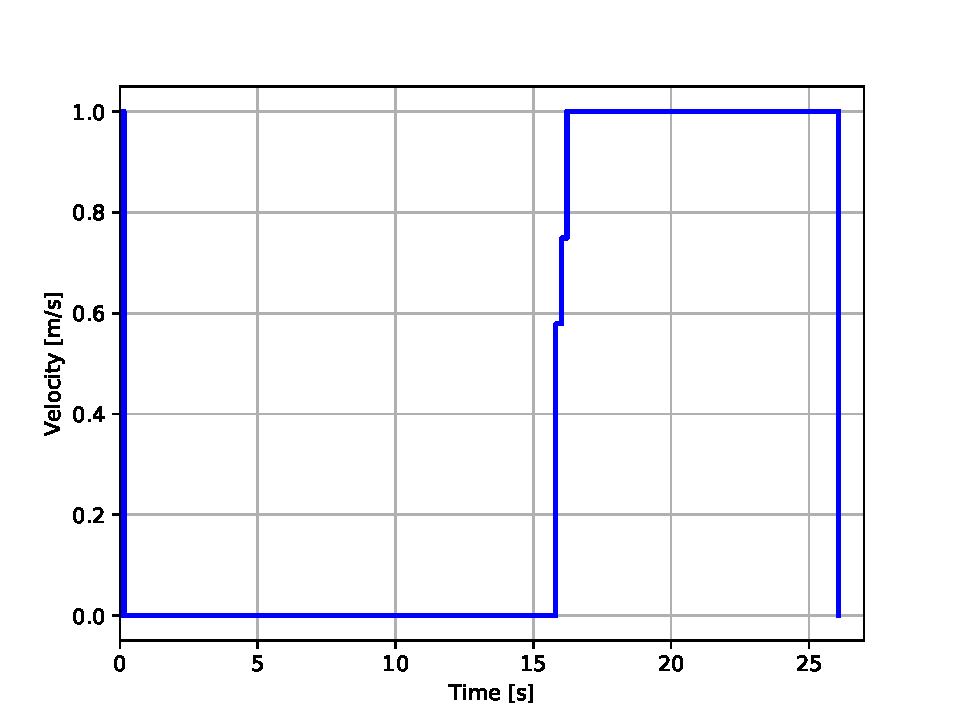
\includegraphics[trim={21 8 40 41}, clip, width=\linewidth]{images/simulations/scene4_2_vel.pdf}
                    \caption{Velocities of the robot during the crossing.}
                \end{subfigure}
                \caption{Results for the fourth scenarion of simulation experiments.}
                \label{fig:scene4_2_graphs}
            \end{figure}
